\documentclass[12pt]{article}

\usepackage{amssymb,amsmath,amsfonts,bbm,eurosym,geometry,ulem,graphicx,caption,color,setspace,sectsty,comment,footmisc,caption,natbib,pdflscape,subfigure,array,hyperref, booktabs, tabularx}

\usepackage[T1]{fontenc}
\usepackage[utf8]{inputenc}
\usepackage{babel}
\usepackage[font=small,labelfont={bf,sf},tableposition=top]{caption}

\normalem

\onehalfspacing
\newtheorem{theorem}{Theorem}
\newtheorem{corollary}[theorem]{Corollary}
\newtheorem{proposition}{Proposition}
\newenvironment{proof}[1][Proof]{\noindent\textbf{#1.} }{\ \rule{0.5em}{0.5em}}

\newtheorem{hyp}{Hypothesis}
\newtheorem{subhyp}{Hypothesis}[hyp]
\renewcommand{\thesubhyp}{\thehyp\alph{subhyp}}

\DeclareMathOperator\erfc{erfc}

\newcommand{\red}[1]{{\color{red} #1}}
\newcommand{\blue}[1]{{\color{blue} #1}}

\newcolumntype{L}[1]{>{\raggedright\let\newline\\arraybackslash\hspace{0pt}}m{#1}}
\newcolumntype{C}[1]{>{\centering\let\newline\\arraybackslash\hspace{0pt}}m{#1}}
\newcolumntype{R}[1]{>{\raggedleft\let\newline\\arraybackslash\hspace{0pt}}m{#1}}

\geometry{left=1.0in,right=1.0in,top=1.0in,bottom=1.0in}

\begin{document}

\begin{titlepage}
\title{A protocol for margining derivatives}
\author{Joseph Clark\thanks{joecmail@gmail.com}  }
\date{\today}
\maketitle
\begin{abstract}
\noindent We give a general construction for margined derivative contracts. This generalises usefully to futures, options, collateralized loans, and state contracts such as prediction markets. For partly collateralized contracts, each side is long an option on their own defaulting and short an option on their counterparty defaulting. Margin insurance and cross margining can be constructed directly with collateralized loans using the margined contract as collateral. 

%In each case we give estimates of the cost of insuring these defaults for realistic scenarios.
% and an expression for the expected value of margin defaults

%\vspace{0in}\\
%\noindent\textbf{Keywords:} key1, key2, key3\\
%\vspace{0in}\\
%\noindent\textbf{JEL Codes:} key1, key2, key3\\

\bigskip
\end{abstract}
\setcounter{page}{0}
\thispagestyle{empty}
\end{titlepage}
\pagebreak \newpage



\doublespacing


\section{Introduction} \label{sec:introduction}

In the absence of legal enforcement of contracts, collateral is required. Some collateralized contracts have enough to satisfy the contract under all circumstances and some only part. Partly collateralized contracts will have enough to cover the immediate liability, a mechanism to monitor collateral value, and a rule for liquidating if this collateral is not forthcoming.

A familiar example is a house loan. A borrower puts up a deposit together with the deed of a house as collateral. The contract will stipulate that the value of the loan cannot exceed some multiple of the value of the house, and the bank will obtain regular valuations to ensure this is the case. If the ratio falls below the contracted amount, the bank will sell the property to satisfy the loan amount and return any remainder to the borrower.

Another example is a margined futures contract. The long and short sides of the contract put up some initial margin at the start of the contract. As the market price of the contract fluctuates, both sides are obliged to maintain a buffer against their liability. If collateral falls below this buffer, the contract is liquidated by finding another party to step into the trade. 

In both examples the structure is of a contract. A well defined payoff structure in the future is traded for some price today. Each side to the contract provides some collateral, and if the collateral falls below an agreed formula the contract is liquidated.

Both sides of the contract face the danger of sharp price moves that make the liability of the contract greater than the collateral. Conceptually these defaults can be modelled as a series of short term options: in each period the price might move before there is a chance to liquidate the contract, and the defaulting side can walk away. 

This paper gives a generic construction of a margining protocol for derivatives that covers common exchange and OTC arrangements. The construction generalises call spreads to European vanilla and binary options, futures, prediction markets, and collateralized loans. 

%The default risk can itself is priced through a collateralized loan secured with the collateral of the contract. These are the same basic construction as a simple collateralized loan, where again the risk is a sequence of forward starting options with a knock out. This can be priced and hedged effectively as a cliquet. 

This construction makes it easy to characterise the risk of margin default explicitly, and in a way that allows margin capital to be imported into a contract by a specialist. Traditional exchanges provide margin insurance as a service. If any trader defaults on margin, the exchange agrees to find another counterparty, and finally to make good on the contract through its own reserves.  This service can be done explicitly as a sequence of contracts covering default for a user using the previous contract as collateral. We provide a construction of this 'Russian Doll' exchange contract in the final section.


\section{A generic margined contract } \label{genericcontracts}

Most  margined contract is defined with 

\begin{itemize}
    \item An underlying state $S(t)$ defined at expiry $T$ and sometimes before
    \item A payoff function at expiry $V(S(T),\ldots)$
    \item Required margin functions for long and short sides of the contract
    $f_m^{i}(\ldots,t),  i = L,S$
    \item Liability functions for long and short sides of the contract $f_l^{i}(\ldots,t),  i = L,S$
    %\item Penalty for breaching margin
    %\[f_h^{i}(\ldots,t),  i = L,S\]
    \item An exchange rate\footnote{Collateral currency for 1 unit of strike currency. The collateral may itself be a contract.} between the strike and collateral currency $m(t)$ 
\end{itemize}

The contract holders put up $C^i(t)$ in collateral. 

Contracts can only be liquidated in some subset $T_L \subseteq [0,T]$. Without losing much generality we use $T_L = (0,1,\ldots,T)$ so liquidation can only occur at the end of each period. If the collateral is less than the margin at any period the contract liquidates by distributing the collateral less the liability 

\begin{equation} \label{defaultpi}
\pi^i(t) = (C^i(t)-f_l^i(t) )^+ 
\end{equation}
%\[(C^i(t)-f_l^i(t) +f_h^i(t))^+\]

%where $f_h^L(t) = -f_h^S(t)$ is a transfer between the long and the short depending on which failed margin.

If both parties maintain sufficient margin to expiry the payoff is 

\begin{equation}\label{expirypi}
\pi^i(T) = C^i(T)-f_l^i(T)
\end{equation}

 

\section{Margin default risk}

Between consecutive liquidation periods the liability might move higher than the collateral value. In this case the contract defaults. The value of this default is a call option on the liability value in $t+1$ with a strike at the collateral value at $t$. 

Figure [X] illustrates with an example of a contract expiring in three periods with a constant amount of collateral. In panel (a) the collateral value is always above the margin and liability so the contract expires and receives a positive payout $C-f_l(3)$. In panel (b) the margin exceeds the collateral in period 2 so the contract liquidates and receives $C-f_l(2)$. In panel (c) the margin and liability exceed collateral and the contract liquidates and receives 0 (the whole collateral $C$ will be released to the other size of the contract).

[Figure]

From the start of the contract, these are sequence of one period forward starting exchange call options options on the liability with a strike a the value of collateral. Each option knocks out if the margin is higher than the the liability for any $t \in T^L$. These can sometimes be priced with reflection-principle based closed form solutions (see \cite{Gaarder02}, \cite{Poulsen06}), but in general the dependence between the liability and posted collateral makes simulation approaches more practical. 

For our purposes the whole default risk is a sequence of these call option payoffs conditioned on the knock-out: 

\begin{equation}
\{\mathbb{I}_{[C(\tau) > f_m(\tau),  \tau<t ]} (f^l(t)-C(t))^+ \}_{t=0}^T  
\end{equation}

Each side is long these call options and short the options of their counterparty in addition to the contracted payoff.

\section{Common contract structures}


\subsection{Futures margined in strike currency} 

Futures are contracts to transact at a specified price in the future. A simple margining scheme for futures requires a fixed dollar variation margin plus/minus changes in contract value.  $\Delta V = V(t)-V(0)$ is the change in contract value between 0 and $t$ and $\delta>0$ is a fixed variation margin. The full contract specification is table \ref{tab:futstrike}.

\begin{table}
\centering
\begin{tabular}{lll|c}
\hline
&  & States & $S(t)$\\
&  & Payoff &  $S(T)$\\
\hline
Long      & margin    & (strike)     & $-\Delta V + \delta$  \\
          &           & (collateral) &\\
          & liability & (strike)     & $-\Delta V$\\
          &           & (collateral)&\\
\hline
Short     & margin    & (strike)     & $\Delta V + \delta$ \\
          &           & (collateral) &\\
          & liability & (strike)     & $\Delta V$\\
          &           & (collateral) &\\          
\hline
\end{tabular}
\caption{Future margined in strike currency.}
\label{tab:futstrike}
\end{table}

%***put itemize envs in tables***
\begin{comment}
\begin{itemize}
    \item State: underlying price $S(t)$
    \item Payoff: $S(T)$
    \item Long margin: $-\Delta V + \delta$
    \item Short margin: $\Delta V + \delta$
    \item Long liability: $-\Delta V$
    \item Short liability: $\Delta V$
\end{itemize}
\end{comment}



\subsubsection*{Example}

$S(0)=V(0)=100$, $\delta=5$. No margin breach penalty.


\textit{Margin breach without default:}
\begin{table}
\begin{tabular}{lll|c|lll}
&  &  &  &  & t &\\  
&  &  &  & 0 & 1 & 2\\
\hline
\hline
&  & States &  $S(t)$ & 100 & 104 & 106\\
&  & Value  &  $V(t)$  & 100 & 104 & 106 \\
&  & Change in value & $\Delta V$ & 0& 4 & 6 \\
\hline
Long      & Margin    & (strike)     & $-\Delta V + \delta$ & 5 & 1 & -1 \\
          &           & (collateral) & & & &\\ 
          & Liability & (strike)     & $-\Delta V$ & 0 & -4 & -6\\ 
          &           & (collateral)& & & &\\
          & Collateral&                       &    & 10 & 10 & 10\\          
\hline          
Short     & Margin    & (strike)     & $\Delta V + \delta$ & 5 & 9 & 11\\
          &           & (collateral) & & & &\\
          & Liability & (strike)     & $\Delta V$ & 0 & 4 & 6\\
          &           & (collateral) & & & &\\
          & Collateral&                       &    & 10 & 10 & 10\\ 
          

\end{tabular}
\caption{Futures in strike currency margin breach without default}
\label{fut}
\end{table}

Initial margin requirement is 5. Long and short contracts put up 10 in strike currency as collateral. Value increases to $V(1) = 104$. Long margin is now -4+5=1 and short margin is 4+5=9. Both contracts are still in margin. Value moves to $V(2)=106$. Short contract breaches margin and contract is liquidated. Long contract gets 16 (initial margin plus variation) and short contract gets 4.


\textit{Margin breach with default:}
\begin{table}
\begin{tabular}{lll|c|lll}
&  &  &  &  & t &\\  
&  &  &  & 0 & 1 & 2\\
\hline
\hline
&  & States &  $S(t)$ & 100 & 115 & \\
&  & Value  &  $V(t)$  & 100 & 115 &  \\
&  & Change in value & $\Delta V$ & 0& 15 &  \\
\hline
Long      & Margin    & (strike)     & $-\Delta V + \delta$ & 5 & -10 & \\
          &           & (collateral) & & & &\\ 
          & Liability & (strike)     & $-\Delta V$ & 0 & -15 & \\ 
          &           & (collateral)& & & &\\
          & Collateral&                       &    & 10 & 10 & \\
\hline          
Short     & Margin    & (strike)     & $\Delta V + \delta$ & 5 & 20 & \\
          &           & (collateral) & & & &\\
          & Liability & (strike)     & $\Delta V$ & 0 & 15 &\\
          &           & (collateral) & & & &\\
          & Collateral&                       &    & 10 & 10 & \\ 
          

\end{tabular}
\caption{Futures in strike currency margin breach with default}
\label{fut}
\end{table}

Initial margin requirement is 5. Long and short contracts put up 10 in strike currency as collateral. Value moves to $V(1) = 115$. Long margin is now -15+5=-10 and short margin is 5+15=20. Short contract breaches margin and defaults. Long contract gets 20 (initial margin plus defaulted collateral) and short contract gets 0. 

\subsection{Collateralized loan}

A collateralized loan has a value function with a single state and different strike and collateral currencies. 

The long contract (borrower) receives $V(0)$ in the strike currency and agrees to repay 1 at expiry. The borrower puts up collateral valued at more than the loan in the collateral currency. As the price of the collateral fluctuates the borrower must maintain the buffer. If this buffer is breached some or all of the collateral is released to the lender to repay the loan. $M_V>1$ is a buffer against movements in the collateral currency exchange rate. The full contract specification is table \ref{tab:loan}.


\begin{table}
\centering
\begin{tabular}{lll|c}
\hline
&  & States & $$\{1\}$\\
&  & Payoff &  $V(T)=S(T)$\\
\hline
Long      & margin    & (strike)     &  \\
          &           & (collateral) & $M_V m(t)(\Delta V + V(0))$\\
          & liability & (strike)     & \\
          &           & (collateral)&$m(t)(\Delta V + V(0))$\\
\hline
Short     & margin    & (strike)     & $V(0)$\\
          &           & (collateral) &\\
          & liability & (strike)     &  $-\Delta V$\\
          &           & (collateral) &\\          
\hline
\end{tabular}
\caption{Collateralized loan}
\label{tab:loan}
\end{table}


\subsubsection*{Example}

$M_V=1.2$, $V(0)=0.9$, $m(0) = 0.1$. No margin breach penalty.

\textit{Margin breach without default:}

Lender puts up 0.9 in strike currency for a one year loan. Margin requirement is 1.2 * 0.1 *0.9 = 0.108 in collateral currency. Borrower puts up 0.15.
$m(1)$ moves to 0.15. $V(1)$ is still 0.9. New margin requirement is 1.2*0.15*0.9 = 0.162 and new liability is 0.15*0.9=0.135. The contract has breached margin. The lender receives 0.135 in collateral to satisfy the loan and the lender receives the remaining 0.015.


\begin{table}
\begin{tabular}{lll|c|lll}
&  &  &  &   & t &\\  
&  &  &  & 0 & 1 & 2\\
\hline
\hline
&  & States &  $S(t)$ & 1 & 1 & \\
&  & Value  &  $V(t)$  & 0.9 & 0.9 &  \\
&  & Change in value & $\Delta V$ & 0& 0 &  \\
\hline
Long      & Margin    & (strike)     &  &  &  &  \\
          &           & (collateral) & $M_V m(t)(\Delta V + V(0))$ & 0.108 & 0.162 &\\ 
          & Liability & (strike)     &  &  &  & \\ 
          &           & (collateral)& $m(t)(\Delta V + V(0))$& 0.09  & 0.135 &\\
          & Collateral&        
          &    & 0.15 & 0.15 & \\ 
\hline          
Short     & Margin    & (strike)     & $V(0)$ & 0.9 & 0.9 & \\
          &           & (collateral) & & & &\\
          & Liability & (strike)     & $-\Delta V$ & 0 & 0 & \\
          &           & (collateral) & & & &\\
          & Collateral&                       &    & 0.9 & 0.9 & \\ 
\hline          

\end{tabular}
\caption{Collateralized loan margin breach without default}
\label{fut}
\end{table}

\textit{Margin breach with default:}

Lender puts up 0.9 in strike currency for a one year loan. Margin requirement is 1.2 * 0.1 *0.9 = 0.108 in collateral currency. Borrower puts up 0.15.
$m(1)$ moves to 0.2. $V(1)$ is still 0.9. New margin requirement is 1.2*0.2*0.9 = 0.216 and new liability is 0.2*0.9=0.18.  The contract has breached margin. The lender receives the full 0.15 in collateral to satisfy the loan and the lender defaults on the remaining 0.03. The lender converts this back to 0.75 in the strike currency and has an 83.33\% recovery rate on the loan. 


\begin{table}
\begin{tabular}{lll|c|lll}
&  &  &  &  & t &\\  
&  &  &  & 0 & 1 & 2\\
\hline
\hline
&  & States &  $S(t)$ & 1 & 1 & \\
&  & Value  &  $V(t)$  & 0.9 & 0.9 &  \\
&  & Change in value & $\Delta V$ & 0& 0 &  \\
\hline
Long      & Margin    & (strike)     &  &  &  &  \\
          &           & (collateral) & $M_V m(t)(-\Delta V + V(0))$ & 0.108 & 0.216 &\\ 
          & Liability & (strike)     &  &  &  & \\ 
          &           & (collateral)& $m(t)(-\Delta V + V(0))$& 0.09  & 0.18 &\\
          & Collateral&                       &    & 0.15 & 0.15 & \\
\hline
Short     & Margin    & (strike)     & $V(0)$ & 0.9 & 0.9 & \\
          &           & (collateral) & & & &\\
          & Liability & (strike)     & $-\Delta V$ & 0 & 0 & \\
          &           & (collateral) & & & &\\
          & Collateral&                       &    & 0.9 & 0.9 & \\ 
\hline          

\end{tabular}
\caption{Collateralized loan margin breach with default}
\label{fut}
\end{table}


\subsection{Futures margined in different currency}

The margin for long and short is held in a different collateral currency. The margins adjust by holding a buffer $M_V>1$ of the strike value.  


\begin{table}
\centering
\begin{tabular}{lll|c}
\hline
&  & States & $$\{1\}$\\
&  & Payoff &  $V(T)=S(T)$\\
\hline
Long      & margin    & (strike)     & \\
          &           & (collateral) & $M_V m(t)(-\Delta V + \delta)$\\
          & liability & (strike)     & \\
          &           & (collateral)& $-m(t) \Delta V$\\
\hline
Short     & margin    & (strike)     & \\
          &           & (collateral) & $M_V m(t)(\Delta V + \delta)$\\
          & liability & (strike)     &  \\
          &           & (collateral) & $m(t)\Delta V$\\          
\hline
\end{tabular}
\caption{Futures margined in different currency}
\label{tab:futcollateral}
\end{table}

\begin{comment}
\begin{itemize} 
    \item State: underlying price $S(t)$
    \item Payoff: $V(T)=S(T)$
    \item Long margin (collateral): $M_V m(t)(-\Delta V + \delta)$
    \item Short margin (collateral): $M_V m(t)(\Delta V + \delta)$
    \item Long liability (collateral): $-m(t) \Delta V$
    \item Short liability (collateral): $m(t)\Delta V$
\end{itemize}
\end{comment}

\subsubsection*{Example}

$S(0)=V(0)=100$, $M_V=1.5$, $m(0)=1$, $\delta=5$. No margin breach penalty.


\textit{Margin breach without default:}


Initial margin requirement is 7.5. Long and short contracts put up 10 in collateral currency. Value increases to $V(1) = 104$ and $m(1)=1$. Long margin is now 1.5 and short margin is 13.5.  The short contract breaches margin. Long contract now gets 14 and short contract gets 6.


\begin{table}
\begin{tabular}{lll|c|lll}
&  &  &  &  & t &\\  
&  &  &  & 0 & 1 & 2\\
\hline
\hline
&  & States &  $S(t)$ & 100 & 104 & \\
&  & Value  &  $V(t)$  & 100 & 104 &  \\
&  & Change in value & $\Delta V$ & 0& 4 &  \\
\hline
Long      & Margin    & (strike)     &  &  &  &  \\
          &           & (collateral) & $M_V m(t)(-\Delta V + \delta)$ & 7.5 & 1.5 &\\ 
          & Liability & (strike)     &  &  &  & \\ 
          &           & (collateral)&$-m(t) \Delta V$ & 0  & -4 &\\
          & Collateral&                       &    & 10 & 10 & \\
\hline
Short     & Margin    & (strike)     &   &  &  & \\
          &           & (collateral) & $M_V m(t)(\Delta V + \delta)$& 7.5 & 13.5 &\\
          & Liability & (strike)     & $-\Delta V$ & 0 & 0 & \\
          &           & (collateral) & $m(t)\Delta V$ & & &\\
          & Collateral&                       &    & 10 & 10 & \\ 
\hline          

\end{tabular}
\caption{Futures margined in different currency margin breach without default}
\label{fut}
\end{table}




\textit{Margin breach with default:}

Initial margin requirement is 7.5. Long and short contracts put up 10 in collateral currency. Value increases to $V(1) = 110$ and $m(1)=2$. Long margin is now -15 and short margin is 45.  The short contract breaches margin. Long contract now gets 20 in collateral and short contract gets 0, having defaulted on 10.


\begin{table}
\begin{tabular}{lll|c|lll}
&  &  &  &  & t &\\  
&  &  &  & 0 & 1 & 2 \\
\hline
\hline
&  & States &  $S(t)$ & 100 & 110 & \\
&  & Value  &  $V(t)$  & 100 & 110 &  \\
&  & Change in value & $\Delta V$ & 0& 10 &  \\
\hline
Long      & Margin    & (strike)     &  &  &  &  \\
          &           & (collateral) & $M_V m(t)(-\Delta V + \delta)$ & 7.5 & -15 &\\ 
          & Liability & (strike)     &  &  &  & \\ 
          &           & (collateral)&$-m(t) \Delta V$ & 0  & -20 &\\
          & Collateral&                       &    & 10 & 10 & \\
\hline
Short     & Margin    & (strike)     &   &  &  & \\
          &           & (collateral) & $M_V m(t)(\Delta V + \delta)$& 7.5 & 45 &\\
          & Liability & (strike)     &  & 0 & 0 & \\
          &           & (collateral) & $m(t)\Delta V$ & 0 & 20 &\\
          & Collateral&                       &    & 10 & 10 & \\ 
\hline          

\end{tabular}
\caption{Futures margined in different currency margin breach with default}
\label{fut}
\end{table}



\subsection{Call spread in strike currency}

Margin for a collateralized call spread can be parameterized with: 

\[ B^L(t) = \min(\delta_1 V(0) + \delta_2, V(0) ) \]

\[ B^S(t) = \min(\delta_1 (K_2-K_1-V(0)) + \delta_2, K_2-K_1-V(0) ) \]

If $\delta_1=1$ and $\delta_2=0$ then the call spread is fully collateralized. The full contract specification is table \ref{tab:callspreadstrike}.

\begin{table}
\centering
\begin{tabular}{lll|c}
\hline
&  & States & $S(t)$ \\
&  & Payoff &  $(S(T)-K_1)^+ -(S(T)-K_2)^+$\\
\hline
Long      & margin    & (strike)     & $-\Delta V + B^L(t)$  \\
          &           & (collateral) &\\
          & liability & (strike)     & $-\Delta V$\\
          &           & (collateral)&\\
\hline
Short     & margin    & (strike)     & $\Delta V + B^S(t)$ \\
          &           & (collateral) &\\
          & liability & (strike)     & $\Delta V$\\
          &           & (collateral) &\\ 
\hline
\end{tabular}
\caption{Call spread in strike currency}
\label{tab:callspreadstrike}
\end{table}

\begin{comment}
\begin{itemize}
    \item State: Single state $S(T)$ 
    \item Payoff: $(S(T)-K_1)^+ -(S(T)-K_2)^+$
    \item Long margin (strike): $-\Delta V + B^L(t)$
    \item Short margin (strike): $\Delta V + B^S(t)$
    \item Long liability (strike): $\Delta V$
    \item Short liability (strike): $-\Delta V$
\end{itemize}
\end{comment}


\subsubsection*{Examples}


$K_1 = 10$, $K_2 = 20$, $S(0)=14$, $\delta_1 =0.2$, $\delta_2= 1$,  $V(0)=4$. No margin breach penalty.

Contract is a call spread between 10 and 20 with current spot at 14. Long and short put up \$1 plus 20\% of maximum loss. Contract initially trades at $\$4$.


Long margin and short margin are

\[f_m^L(\ldots,t) = -\Delta V + \min(0.2 V(0) + 1, V(0))\]

\[f_m^S(\ldots,t) = \Delta V + \min(0.2 (10-V(0)) + 1, 10 - V(0))\]

\textit{Margin breach without default:}


Long contract required margin is $0.2 *(4) + 1 = 1.8$. Short contract required margin is $0.2 *(6)+ 1 = 2.2$. Both contracts put up $2.5$ in collateral.
$V(1)$ moves to 5. Long contract required margin is $-1+0.2*(5) +1 = 1$. Short contract required margin is $ 1 + 0.2*(5)+ 1 = 3$. Short contract breaches margin. Short contract receives $2.5 +1 = 3.5$ and long contract receives $2.5 - 1 = 1.5$.

\begin{table}
\begin{tabular}{lll|c|lll}
&  &  &  &  & t &\\  
&  &  &  & 0 & 1 & 2\\
\hline
\hline
&  & States &  $S(t)$ & 14 & 16 & \\
&  & Value  &  $V(t)$  & 4 & 5 &  \\
&  & Change in value & $\Delta V$ & 0& 1 &  \\
\hline
Long      & Margin    & (strike)     & $-\Delta V + B^L(t)$ & 1.8 & 1 &  \\
          &           & (collateral) & & & &\\ 
          & Liability & (strike)     & $-\Delta V$ & 0 & -1 & \\ 
          &           & (collateral)& & & &\\
          & Collateral&                       &    & 2.5 & 2.5 & \\          
\hline          
Short     & Margin    & (strike)     & $\Delta V + B^S(t)$  & 2.2 & 3 & \\
          &           & (collateral) & & & &\\
          & Liability & (strike)     & $\Delta V$ & 0 & 1 & \\
          &           & (collateral) & & & &\\
          & Collateral&                       &    & 2.5 & 2.5 & \\ 
          

\end{tabular}
\caption{Call spread in strike currency margin breach without default}
\label{fut}
\end{table}



\textit{Margin breach with default:}

Long contract required margin is $0.2 *( 4) + 1 = 1.8$. Short contract required margin is $0.2 *( 6 )+ 1 = 2.2$. Both contracts put up $2.5$ in collateral.
$V(1)$ moves to 8. Long contract required margin is $-4+0.2*(8) +1 = -1.4$.  Short contract required margin is $ 4 + 0.2*(2)+ 1 = 5.4$. Short contract breaches margin and defaults. Short contract receives $5$ and long contract receives $0$.

\begin{table}
\begin{tabular}{lll|c|lll}
&  &  &  &  & t &\\  
&  &  &  & 0 & 1 & 2\\
\hline
\hline
&  & States &  $S(t)$ & 14 & 19 & \\
&  & Value  &  $V(t)$  & 4 & 8 &  \\
&  & Change in value & $\Delta V$ & 0& -4 &  \\
\hline
Long      & Margin    & (strike)     & $-\Delta V + B^L(t)$ & 1.8 & -1.4 &  \\
          &           & (collateral) & & & &\\ 
          & Liability & (strike)     & $-\Delta V$ & 0 & -4 & \\ 
          &           & (collateral)& & & &\\
          & Collateral&                       &    & 2.5 & 2.5 & \\          
\hline          
Short     & Margin    & (strike)     & $\Delta V + B^S(t)$  & 2.2 & 5.4 & \\
          &           & (collateral) & & & &\\
          & Liability & (strike)     & $\Delta V$ & 0 & 4 & \\
          &           & (collateral) & & & &\\
          & Collateral&                       &    & 2.5 & 2.5 & \\ 
          

\end{tabular}
\caption{Call spread in strike currency margin breach with default}
\label{fut}
\end{table}


\subsection{Call in strike currency}

A call is a call strike with $K_2=\infty$. Margin for a collateralized call spread can be parameterized with: 

\[ B^L(t) = \min(\delta_1 V(0) + \delta_2, V(0)) \]

\[ B^S(t) = \max(\delta_3 S(t) \delta_4 (S(t)-K), V(0)) \]

The long call option holder puts up as margin some fraction of the premium plus a fixed value. The short option puts up a fraction of the underlying and a fraction of payoff if the option were to expire today.  The full contract specification is table \ref{tab:callstrike}

\begin{table}
\centering
\begin{tabular}{lll|c}
\hline
&  & States & $S(t)$\\
&  & Payoff &  $(S(T)-K)^+$\\
Long      & margin    & (strike)     & $-\Delta V + B^L(t)$  \\
          &           & (collateral) &\\
          & liability & (strike)     & $-\Delta V$\\
          &           & (collateral)&\\
Short     & margin    & (strike)     & $\Delta V + B^S(t)$ \\
          &           & (collateral) &\\
          & liability & (strike)     & $\Delta V$\\
          &           & (collateral) &\\          
\hline
\end{tabular}
\caption{Call option in strike currency}
\label{tab:callstrike}
\end{table}

\begin{comment}
\begin{itemize}
    \item State: Single state $S(T)$ 
    \item Payoff: $(S(T)-K)^+$
    \item Long margin (strike): $-\Delta V + B^L(t)$
    \item Short margin (strike): $\Delta V + B^S(t)$
    \item Long liability (strike): $\Delta V$
    \item Short liability (strike): $-\Delta V$
\end{itemize}
\end{comment}


\subsubsection*{Examples}

$S(0)=100$, $K=110$, $T$= 1 year, $\delta_1=1$, $\delta_2=0$, $\delta_3 =0.1$, $\delta_4=0$, $V(0)=10$


\textit{Margin breach without default:}

Long contract required margin is $10$. Short contract required margin is $10$. Long contract posts 10. Short contract posts 11. $S(1)$ moves to 110. $V(1)$ moves to 15. Long contract required margin is $-5 + 15=10$ Short contract required margin is $5 + 0.1*110 = 16$. Short contract breaches margin. Long contract receives 15 and short contract receives $11-5=6$.


\begin{table}
\begin{tabular}{lll|c|lll}
&  &  &  &  & t &\\  
&  &  &  & 0 & 1 & 2\\
\hline
\hline
&  & States &  $S(t)$ & 100 & 110 & \\
&  & Value  &  $V(t)$  & 10 & 15 &  \\
&  & Change in value & $\Delta V$ & 0& 5 &  \\
\hline
Long      & Margin    & (strike)     & $-\Delta V + B^L(t)$& 10 & 10 & \\
          &           & (collateral) & & & &\\ 
          & Liability & (strike)     & $-\Delta V$ & 0 & -5 & \\ 
          &           & (collateral)& & & &\\
          & Collateral&                       &    & 10 & 10 & \\
\hline          
Short     & Margin    & (strike)     & $\Delta V + B^S(t)$ & 10 & 16 & \\
          &           & (collateral) & & & &\\
          & Liability & (strike)     & $\Delta V$ & 0 & 5 &\\
          &           & (collateral) & & & &\\
          & Collateral&                       &    & 11 & 11 & \\ 
          

\end{tabular}
\caption{Call option in strike currency margin breach without default}
\label{fut}
\end{table}


\textit{Margin breach with default:}


Long contract required margin is $10$. Short contract required margin is $10$. Long contract posts 10. Short contract posts 11. $S(1)$ moves to 120. $V(1)$ moves to 25. Long contract required margin is $-15 + 25= 10$. Short contract required margin is $ 15+ 0.1*120 = 27$. Short contract breaches margin. Short contract receives 20 and long contract receives $0$, having defaulted 4.


\begin{table}
\begin{tabular}{lll|c|lll}
&  &  &  &  & t &\\  
&  &  &  & 0 & 1 & 2\\
\hline
&  & States &  $S(t)$ & 100 & 120 & \\
&  & Value  &  $V(t)$  & 10 & 25 &  \\
&  & Change in value & $\Delta V$ & 0& 15 &  \\
\hline
\hline
Long      & Margin    & (strike)     & $-\Delta V + B^L(t)$& 10 & 10 & \\
          &           & (collateral) & & & &\\ 
          & Liability & (strike)     & $-\Delta V$ & 0 & -15 & \\ 
          &           & (collateral)& & & &\\
          & Collateral&                       &    & 10 & 10 & \\
\hline          
Short     & Margin    & (strike)     & $\Delta V + B^S(t)$ & 10 & 27 & \\
          &           & (collateral) & & & &\\
          & Liability & (strike)     & $\Delta V$ & 0 & 15 &\\
          &           & (collateral) & & & &\\
          & Collateral&                       &    & 11 & 11 & \\ 
          

\end{tabular}
\caption{Call option in strike currency margin breach with default}
\label{fut}
\end{table}

\subsection{Event market in strike currency}

An event market is a future with two possible states. Margin can be parameterized with:


\[ B^L(t) = \min(\delta_1 V(0) + \delta_2, V(0) ) \]

\[ B^S(t) = \min(\delta_1 (1-V(0)) + \delta_2, 1-V(0) ) \]

If $\delta_1=1$ and $\delta_2=0$ the contract is fully collateralized.


\begin{table}
\centering
\begin{tabular}{lll|c}
\hline
&  & States & $S(T) \in \{0,1\}$ \\
&  & Payoff &  $S(T)$\\
Long      & margin    & (strike)     & $-\Delta V + B^L(t)$  \\
          &           & (collateral) &\\
          & liability & (strike)     & $-\Delta V$\\
          &           & (collateral)&\\
Short     & margin    & (strike)     & $\Delta V + B^S(t)$ \\
          &           & (collateral) &\\
          & liability & (strike)     & $\Delta V$\\
          &           & (collateral) &\\          
\hline
\end{tabular}
\caption{Call option in strike currency}
\label{tab:eventstrike}
\end{table}

\begin{comment}
\begin{itemize}
    \item State: Single state $S(T) \in \{0,1\}$ 
    \item Payoff: $S(T)$
    \item Long margin (strike): $-\Delta V + B^L(t)$
    \item Short margin (strike): $\Delta V + B^S(t)$
    \item Long liability (strike): $\Delta V$
    \item Short liability (strike): $-\Delta V$
\end{itemize}
\end{comment}



\subsubsection*{Examples}

$V(0)=0.3$, $\delta_1=0.2$, $\delta_2=0.1$. 


\textit{Margin breach without default:}


Long contract required margin is $0.2*0.3 +0.1 = 0.16$. Short contract required margin is $0.2*0.7 +0.1 = 0.24$. Long contract posts 0.2. Short contract posts 0.3. $V(1)$ moves to 0.5. Long contract required margin is $-0.2+0.2*0.5 + 0.1 = 0$. Short contract required margin is $0.2+0.2*0.5 + 0.1 = 0.4$
Short contract breaches margin. Long contract receives 0.5 and short contract receives $0$.


\begin{table}
\begin{tabular}{lll|c|lll}
&  &  &  &  & t &\\  
&  &  &  & 0 & 1 & 2\\
\hline
\hline
&  & States &  $S(t)$ &   &   & \\
&  & Value  &  $V(t)$  & 0.3 & 0.5 &  \\
&  & Change in value & $\Delta V$ & 0& 0.2 &  \\
\hline
Long      & Margin    & (strike)     & $-\Delta V + B^L(t)$& 0.16 & 0 & \\
          &           & (collateral) & & & &\\ 
          & Liability & (strike)     & $-\Delta V$ & 0 & -0.2 & \\ 
          &           & (collateral)& & & &\\
          & Collateral&                       &    & 0.2 & 0.2 & \\
\hline          
Short     & Margin    & (strike)     & $\Delta V + B^S(t)$ & 0.24 & 0.4 & \\
          &           & (collateral) & & & &\\
          & Liability & (strike)     & $\Delta V$ & 0 & 0.2 &\\
          &           & (collateral) & & & &\\
          & Collateral&                       &    & 0.3 & 0.3 & \\ 
          

\end{tabular}
\caption{Event market in strike currency margin breach without default}
\label{fut}
\end{table}


\textit{Default:}

Long contract required margin is $0.2*0.3 +0.1 = 0.16$.  Short contract required margin is $0.2*0.7 +0.1 = 0.24$. Long contract posts 0.2. Short contract posts 0.3. $V(1)$ moves to 0.7. Long contract required margin is $-0.4+0.2*0.7 + 0.1 = -0.16$. Short contract required margin is $0.4+0.2*0.3 + 0.1 = 0.56$. Short contract breaches margin. Long contract receives 0.5 and short contract receives $0$, having defaulted 0.1.

\begin{table}
\begin{tabular}{lll|c|lll}
&  &  &  & t & &\\  
&  &  &  & 0 & 1 & 2\\
\hline
&  & States &  $S(t)$ &   &   & \\
&  & Value  &  $V(t)$  & 0.3 & 0.7 &  \\
&  & Change in value & $\Delta V$ & 0& 0.4 &  \\
\hline
Long      & Margin    & (strike)     & $-\Delta V + B^L(t)$& 0.16 & -0.16 & \\
          &           & (collateral) & & & &\\ 
          & Liability & (strike)     & $-\Delta V$ & 0 & -0.4 & \\ 
          &           & (collateral)& & & &\\
          & Collateral&                       &    & 0.2 & 0.2 & \\
\hline          
Short     & Margin    & (strike)     & $\Delta V + B^S(t)$ & 0.24 & 0.56 & \\
          &           & (collateral) & & & &\\
          & Liability & (strike)     & $\Delta V$ & 0 & 0.4 &\\
          &           & (collateral) & & & &\\
          & Collateral&                       &    & 0.3 & 0.3 & \\ 
          
\end{tabular}
\caption{Event market in strike currency margin breach with default}
\label{fut}
\end{table}



\section{Contracts as collateral}

Using contracts as collateral does not change the process of margining, though important differences arise depending on 

\subsection{Embedded value loans}

Imagine a contract that has a large amount of embedded value -- say, an in-the-money option close to expiry. The holder of the contract takes out a loan using the contract as collateral. The effect is to reduce the margin requirement by substituting loan collateral. 

This  arrangement is simply a collateralized loan (see above) where the collateral currency is the original contract. If the value of the contract reduces too close to the value of the loan, the lender takes a portion of the contract in fulfillment of the loan and returns the remainder to the borrower.

\subsection{Insurance as chained collateral contracts}

The idea of an insurance market is to use a single collateral pool to insure multiple risks. Provided that the bad outcomes do not happen at once, there will be enough to satisfy all the liabilities. Insurers like to have a portfolio of houses in different geographies so that a particular earthquake or hurricane does not wipe out their reserves.

We can implement pure pooling in generic contracts of section \ref{genericcontracts} by specifying a value function. Either paying the whole claim of each or scaling down each claim to match the available liquidity. The problem with this approach is that each new insurance contract dilutes the effectiveness of previous contracts. An unscrupulous insurer might sell too much insurance and be wiped out in a way that policy holders cannot foresee or control.

One solution is to have each new policy sold with its full liabilities visible, and have that contract be collateral for the next contract. Prospective insurance purchasers can inspect the contract and construct their own model of the value of the promise given the more senior liabilities.

Alice locks \$100 in a contract and insures Bob for a year for up to \$10 of earthquake damage. Alice uses her claim to this contract as collateral to sell  \$90 of hurricane insurance to Carol, and that contract as collateral to insure Dave's car for \$50. Bob and Carol's are confident their claims will be met. The value of Dave's cover will depend on the likelihood of earthquakes and hurricanes, and his relatively lower insurance premium will reflect this. 


\subsection{Pooled margin insurance as a service}

Exchanges provide a useful service being the counterparty to all trades. If a contract has insufficient margin the exchange will try to find a new counterparty from its stable of market makers and ultimately take on the contract against the its own reserves. This arrangement works well, but traders cannot know much about the default risk the exchange will hold in the future. 

The exchange contract can be deconstructed as a chained insurance contract as in the previous section. The exchange contract starts with some collateral and contracts to make good on margin defaults for a single period. This contract (the collateral and the first contract) is used as collateral for a second contract. At each stage the purchaser can see all the previous (and more senior) contracts.

Such margin insurance could conceivably re-contracted over short periods of time with multiple exchange pools providing quotes for margin insurance in each period, and buyers choosing on price and risk according to a rule. An interface could be put in front of this so it would seem like an ordinary margined exchange for a trader.

\section{Pricing results}

\section{Estimated cost of margin defaults}

\subsection*{Data}
We use Bitcoin/USD exchange data from Bitfinex with a one minute increment from 1 May 2013 to 23 November 2020. 

\subsection*{Methodology}
We simulate defaults on several contracts assuming that the margin is posted at the start of each period and liquidation is only possible on the minute. 

The default value for each minute is the any liability more than the margin over the minute as a fraction of the state value: 

\begin{equation} \label{default_est}
default(t) = \frac{(f_l^i(t)- m^i(t-1) )^+}{S(t-1)}
\end{equation}

Figure \ref{fig:FutMarginDefaultCost} has the annualized average cost of defaults for margin collateral between 10\% and 50\% of the underlying value. 

The larger default-inducing moves are in 2013 and 2014, we also show results for the 2015-2020 sample. 

\begin{figure}
    \centering
    \subfigure[Full sample]{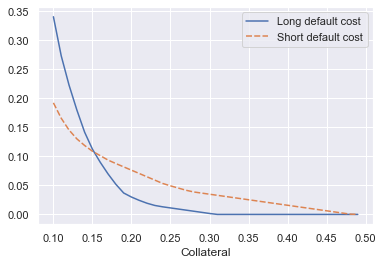
\includegraphics[width=0.7\textwidth]{figs/FutMarginDefaultCost.png}}
    \subfigure[2015-2020]{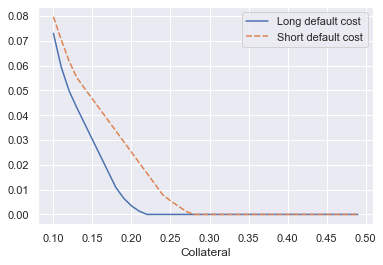
\includegraphics[width=0.7\textwidth]{figs/FutMarginDefaultCost_post2015.png}}
    \caption{BTC/USD margined futures default insurance cost (annualized) 2013-2020 }
    \label{fig:FutMarginDefaultCost}
    
\end{figure}











\begin{thebibliography}{}


\bibitem{Gaarder02} Esben Gaarder Haug and Jørgen Haug. Knock-in/out Margrabe. Wilmott Magazine, 1(December):38–41, 2002

\bibitem{Poulsen06} Rolf Poulsen. Barrier Options and Their Static Hedges: Simple Derivations and
Extensions. Quantitative Finance, 6:327–335, 2006.


%\bibitem{Jac2010} Jacobs, Kurt (2010). Stochastic Processes for Physicists. Cambridge University Press. pp. 57–59

%\bibitem{Merton73} Merton, Robert (1973). \textit{Theory of Rational Option Pricing}. Bell Journal of Economics and Management Science. 4 (1): 141–183.


%@article{angeris2019analysis,
%  title={An analysis of Uniswap markets},
%  author={Angeris, Guillermo and Kao, Hsien-Tang and Chiang, Rei and Noyes, %Charlie and Chitra, Tarun},
%  journal={arXiv preprint arXiv:1911.03380},
%  year={2019}


\end{thebibliography}

\end{document}
